\documentclass[12pt,a4paper]{article}

\usepackage{amsmath}
\usepackage{amssymb}
\pagestyle{empty}
\usepackage[margin=1in]{geometry}
\usepackage{hyperref}
\usepackage[utf8]{inputenc}
\usepackage[IL2]{fontenc}
\usepackage[czech]{babel}
\usepackage{amsthm}
\usepackage{enumitem}
\usepackage{graphicx}

\theoremstyle{definition}
\newtheorem{uloha}{Úloha}

\DeclareMathOperator{\tg}{tg}
\def\ee{\mathrm{e}}

%\setlist[enumerate]{label={(\alph*)}}

\begin{document}

\section*{Slovní úlohy na derivace!}
%\bigskip

%Výsledky jsou na druhé straně.

\begin{uloha}
Součet dvou reálných čísel je $20$. Jaký největší může být jejich součin?
\end{uloha}

\begin{uloha}
Součin dvou reálných čísel je $20$.
\begin{enumerate}[label={(\alph*)}]
	\item Jaký je jejich nejmenší možný součet, pokud se omezíme jen na kladná čísla?
	\item Jaký je jejich nejmenší možný součet?
	\item Jaký je jejich největší možný součet?
\end{enumerate}
\end{uloha}


\begin{uloha}
Farmář chce postavit obdélníkový plot, který bude dále pletivem rozdělen na tři obdélníkové podoblasti o stejných rozměrech (zhruba jako na obrázku). K dispozici má 1000\,m pletiva. Jaký největší obsah může oplocené území mít?
\[ 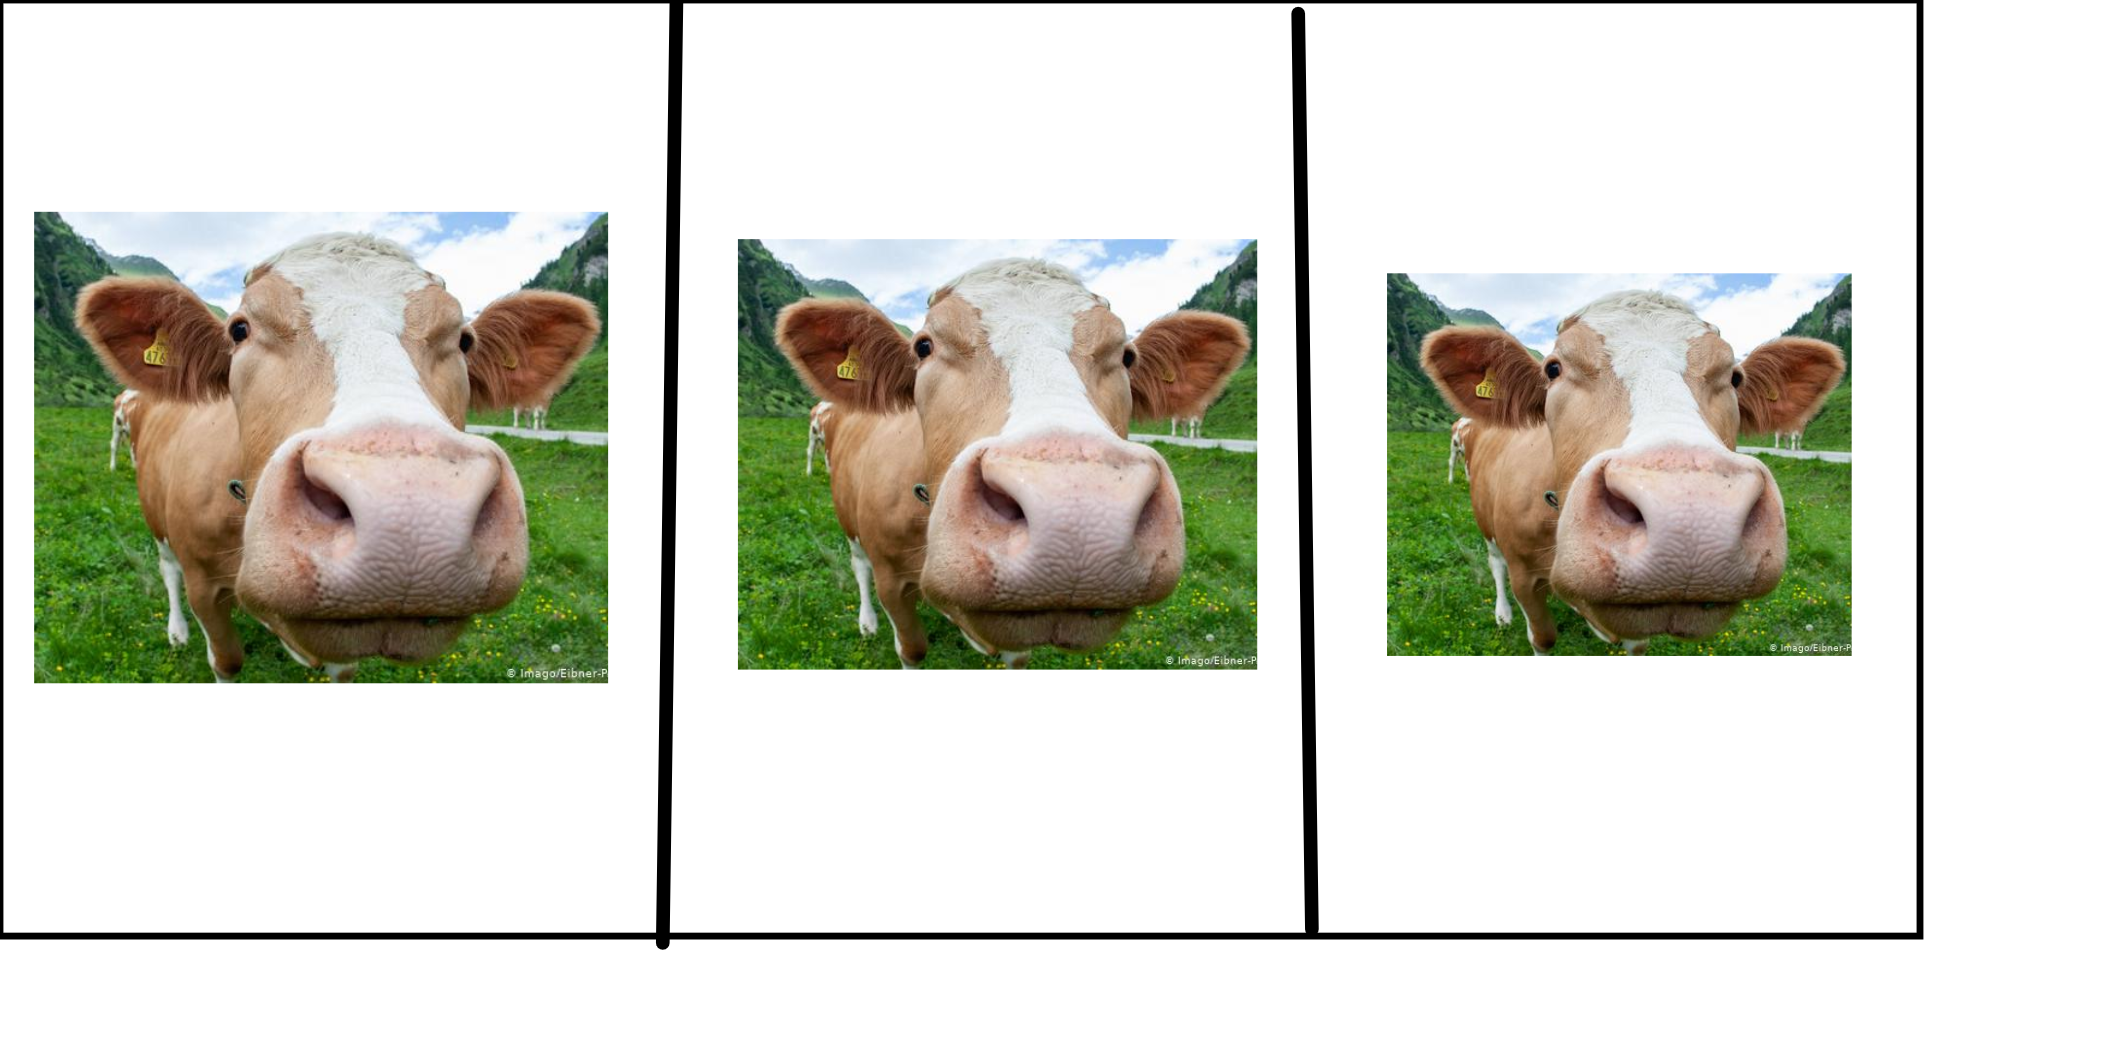
\includegraphics[width=6cm]{kravy.png} \]
\end{uloha}


\begin{uloha}
Letadlo $A$ se nachází na souřadnicích $[0; 8]$, letadlo $B$ na $[7; 0]$. Obě letadla se pohybují rovnoměrně přímočaře, přičemž $A$ se pohybuje rychlostí $1$ tak, že klesá jeho $y$-ová souřadnice, zatímco $B$ se pohybuje rychlostí $2$ tak, že klesá jeho $x$-ová souřadnice. V jaký moment budou k sobě nejblíže?
\end{uloha}


\begin{uloha}
Dva zářiče jsou od sebe vzdáleny třicet metrů, přičemž poměr jejich výkonů je $27:8$. Intenzita ozáření klesá s druhou mocninou vzdálenosti od zářiče. Jaké místo na spojnici obou zářičů (které považujeme za body) je v součtu ozářeno nejméně?
\end{uloha}


\begin{uloha}
Nalezněte nejkratší cestu z bodu $A[0; 1]$ do bodu $B[5; 3]$, která se dotkne osy $x$.
\end{uloha}


\begin{uloha}
Kometa se pohybuje po parabole o rovnici $y = x^2$. V jakém bodě bude nejblíže asteroidu o souřadnicích $[3; 0]$? Možná bude potřeba vyřešit nějakou kubickou rovnici, tak si vhodně pomožte stroji (nebo zkuste její řešení tipnout).
\end{uloha}


\begin{uloha}
Máme kus drátu (dlouhý např. 10\,cm), který můžeme přestřihnout, z jedné části vyrobit čtverec a z druhé obdélník s poměrem stran $1:3$. Jak máme drát přestřihnout, aby byl celkový obsah výsledných útvarů
\begin{enumerate}[label={(\alph*)}]
	\item co nejmenší?
	\item co největší?
\end{enumerate}
\end{uloha}

\begin{uloha}
Z obdélníkového listu papíru o rozměrech $10\times 20$ chceme vystřihnout čtvercové rohy a výsledek poohýbat na kvádr, kterému bude chybět jedna stěna. Jak velké rohy vystřinout, aby měl výsledek co největší objem?
\end{uloha}

\begin{uloha}
Naším úkolem je navrhnout kontejner s tvarem kvádru, jehož spodní stěna má poměr stran $1:2$, a objemem $10\,$m$^3$, který bude nahoře odklopený. Za každý m$^2$ podstavy spotřebujeme materiál za 1000\,Kč a za m$^2$ boční stěny jen 600\,Kč. Jaké rozměry bude mít nejlevnější varianta?
\end{uloha}


%\end{document}

\newpage

\subsection*{Výsledky}

%\setcounter{uloha}{0}


%\begin{uloha}
\begin{enumerate}%[label={\arabic*.}]
	\item $100$
	\item (a) $4 \sqrt5$, (b) když připustíme záporné hodnoty, tak může být libovolně malý, (c) může být libovolně velký.
	\item $31250\,$m$^2$ (rozměry $250\times 125$)
	\item 4,4 jednotek času od současné chvíle
	\item 18\,m od silnějšího zdroje
	\item je to cesta vedoucí přes $[5/4; 0]$
	\item $[1; 1]$
	\item (a) čtverec vyrobíme z kusu dlouhého $\frac{30}{7}$\,cm, (b) vůbec nestříhat a sestrojit čtverec z jednoho kusu
	\item rohy o straně $\frac{5}{3} \left(3-\sqrt{3}\right)$
	\item spodní strana má rozměry $\sqrt[3]{9/2} \times 2\sqrt[3]{9/2}$, výška pak je $\frac53 \cdot \sqrt[3]{\frac43}$
\end{enumerate}
%\end{uloha}
%
%
%\begin{uloha}
%
%\end{uloha}

\end{document}